\section{Camera Calibration}
We started out by calibrating the camera using a chessboard pattern provided by the OpenCV library. This allowed us to compute both, intrinsic and extrinsic camera parameters as well as distortion coefficients for the camera. 

\begin{equation}
	P = K \begin{bmatrix} R|t \end{bmatrix}
\end{equation}

The intrinsic camera parameters \textit{K} do not change in time, because the camera we used does not have the ability to change the focal length of the lens, so it makes sense to store this data for later. 

The extrinsic parameters (\textit{R} and \textit{t}) on the other hand change with the position of the chessboard pattern.

Intrinsic and extrinsic parameters together make camera projection matrix \textit{P}. We use this matrix later to calculate homography between the first view we used to store the camera calibration and subsequent views in the rendering.

To verify that \textit{P} is correct we projected chess points on the first camera view. As you can see in the Figure \ref{subfig:chesspattern} all the points have been projected exactly into the right position.
 
 \begin{figure}[h!]
	\begin{subfigure}[b]{0.5\textwidth}
		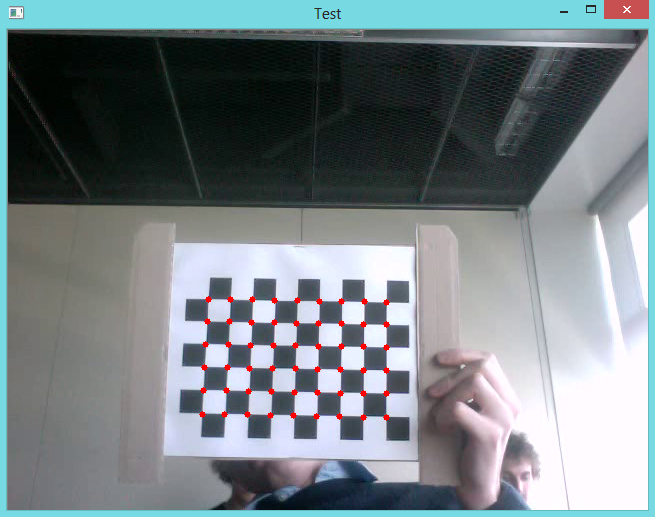
\includegraphics[width=\textwidth]{Handin3/images/patterndot.jpg}
		\caption{Chessboard}
		\label{subfig:chesspattern}
	\end{subfigure}
	~
	\begin{subfigure}[b]{0.5\textwidth}
		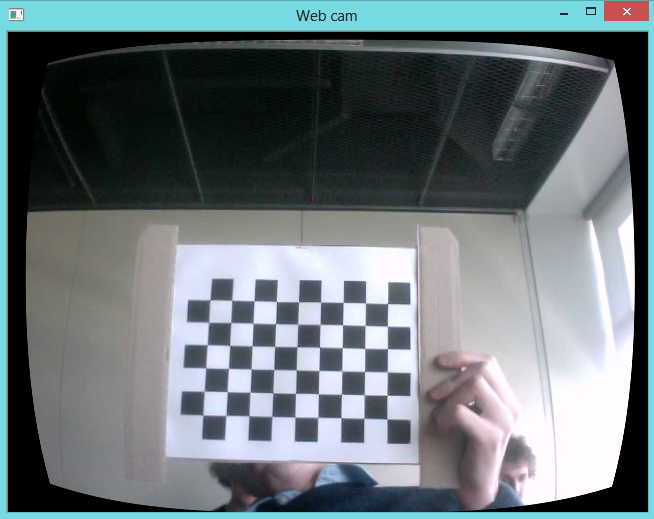
\includegraphics[width=\textwidth]{Handin3/images/undistort.jpg}
		\caption{Undistort}
		\label{subfig:undistort}
	\end{subfigure}
	
	\caption{Camera Calibration}
\end{figure}
 
In the last step of this part we tried to undistort the image by using the (cv2.undistort) function. (see Figure \ref{subfig:undistort}). Using the chessboard, OpenCV has been able to calculate camera distortion coefficients, that we have stored for later use as well.

 
